\chapter{Fundamentação Teórica}
\label{cap:fundamentacao-teorica}

% Alguns autores preferem fazer uma ``fundamentação teórica'' no segundo capítulo, outros, preferem fazer uma ``revisão da literatura''. Entretanto, isto é particular de cada trabalho e o autor deve escolher o título mais adequado para o capítulo. Consultar o orientador é importante para determinar o título apropriado.

% Evite começar da seção secundária, ou seja, não passe direto do título do capítulo para o título da seção secundária. Escreva um texto para introduzir as seções subsequentes. Lembre-se de utilizar primeira letra maiúscula quando estiver se referindo a um objeto com numeração específica como capítulo, seção, subseção, figura, tabela, quadro, equação, normalmente, se escreve a primeira letra maiúscula da palavra do objeto seguido do \textit{label}. Por exemplo, a Seção \ref{sec:citacoes} explica como fazer citações bibliográficas. Observe no código fonte deste texto como foi feita a referência cruzada. Isso permite enumerar a seção do modo automático o que facilita caso novas seções sejam criadas.  

Neste capítulo será introduzido a definição de sistemas embarcados, bem como alguns de seus tipos, diferenças arquiteturais e quais aplicações se encaixam melhor a cada um desses tipos de sistema. Em seguida, será apresentado a definição de Sistemas de Aquisição de Dados - DAQs, e \textit{Dataloggers}, aplicações e diferenças entre eles.





\section{Sistemas Embarcados}\label{sec:definicao_sistemas_embarcados}

\subsection{Definição}

Sistemas computacionais são normalmente associados a grandes computadores de centros de processamento de dados, computadores de mesa e afins. Contudo, devido a miniaturização de componentes eletrônicos, esses sistemas puderam ser reduzidos ao ponto de fazerem parte da construção de diversos produtos do cotidiano. Impressoras, máquinas registradoras, controles remotos são alguns exemplos desses produtos. Dessa forma, para sistemas computacionais que são parte integrante de um produto ou ferramenta é dado a denominação de sistemas embarcados.

\subsection{Características}






\subsection{Propriedades}



\subsection{Aplicações}








\section{Dataloggers}\label{sec:datalogger}



\section{\textit{Data Acquisition Systems} - DAQs}

\if{0}
    % Esta frase mostra como citar um livro sobre descargas atmosféricas \cite{rakov2003lightning}. Também podem ser citados \textit{sites} como \citeonline{elat2015densidade}. Você precisa escrever o código da referência no arquivo "referencia.bib" dentro da pasta "elementos-pos-textuais". Veja esse, onde estão alguns exemplos que já foram testados.        

    Referenciando outro livro \cite{LangtangenLogg2017}. Texto texto texto texto texto texto texto texto texto texto texto texto texto texto texto texto texto texto texto. Texto texto texto texto texto texto texto texto texto texto texto texto texto texto texto texto texto texto texto. Texto texto texto texto texto texto texto texto texto texto texto texto texto texto texto texto texto texto texto. Texto texto texto texto texto texto texto texto texto texto texto texto texto texto texto texto texto texto texto.

    Referenciando outro site \cite{secretaria1999}. Texto texto texto texto texto texto texto texto texto texto texto texto texto texto texto texto texto texto texto. Texto texto texto texto texto texto texto texto texto texto texto texto texto texto texto texto texto texto texto. Texto texto texto texto texto texto texto texto texto texto texto texto texto texto texto texto texto texto texto. Texto texto texto texto texto texto texto texto texto texto texto texto texto texto texto texto texto texto texto. Citando uma norma \cite{NBR10520:2002}.
        
    Citação de duas referências que concordam entre si \cite{Almeida2018,Gondim2017}. Texto texto texto texto texto texto texto texto texto texto texto texto texto texto texto texto texto texto texto. Texto texto texto texto texto texto texto texto texto texto texto texto texto texto texto texto texto texto texto. Texto texto texto texto texto texto texto texto texto texto texto texto texto texto texto texto texto texto texto. Texto texto texto texto texto texto texto texto texto texto texto texto texto texto texto texto texto texto texto texto texto texto texto texto texto texto. Citando um manual \cite{manuais1989}. 
        
    Outro tipo de citação é a citação literal ou direta com mais de três linhas. Este tipo de citação deve ser destacada com recuo de $4~cm$ da margem esquerda com letra menor (tamanho 10), sem aspas e com espaçamento simples.  Para exemplificar esse tipo de citação, considere a afirmação de \citeonline{feitosa2016}:
    \begin{citacao}
        A cultura é o processo através do qual o homem cria o algo onde antes imperava o nada. Esse algo é toda complexidade de criações simbólicas, de sentidos e significados que damos às coisas e ao mundo. Um ``algo'' que não se sustenta se não se entender os processos culturais como mecanismos de mediação entre nós e os fenômenos. Assim, mais do que apenas um elemento da comunicação, a mediação é, por excelência, cultural. As diversas modalidades de mediação são apenas sotaques diferenciados dessa mediação cultural. Assim é a mediação informacional.
    \end{citacao}
        
    A afirmação do parágrafo anterior também pode ser reproduzida com a citação na final como mostra o exemplo a seguir: 
    \begin{citacao}
        A cultura é o processo através do qual o homem cria o algo onde antes imperava o nada. Esse algo é toda complexidade de criações simbólicas, de sentidos e significados que damos às coisas e ao mundo. Um “algo” que não se sustenta se não se entender os processos culturais como mecanismos de mediação entre nós e os fenômenos. Assim, mais do que apenas um elemento da comunicação, a mediação é, por excelência, cultural. As diversas modalidades de mediação são apenas sotaques diferenciados dessa mediação cultural. Assim é a mediação informacional. \cite{feitosa2016}.
    \end{citacao}
        
%Mais exemplos e opções de citações podem ser encontradas em:
%        https://en.wikibooks.org/wiki/LaTeX/Bibliography_Management
%        https://github.com/cfgnunes/latex-cefetmg/blob/master/latex-cefetmg/03-elementos-pos-textuais/apendices.tex            

\section{Inserindo figuras}\label{sec:figuras}
    
    A Figura \ref{fig:reitoria} apresenta a fotografia da reitoria da Universidade Federal do Ceará. Observe a estrutura do código para ver como inserir figuras. No título, comece especificando o tipo de figura. Por exemplo, fotografia, desenho, diagrama, fluxograma, gráfico e etc. O espaçamento entre linhas no título é de $1~pt$ (espaçamento simples), apenas a primeira letra da frase é maiúscula. As demais palavras são escritas com letra maiúsculas somente quando são nomes próprios e não há ponto final. 
    
    As margens do título da figura são delimitadas pelo tamanho da figura. Por isso, procure ajustar o tamanho da figura para preencher a largura delimitada pelas margens esquerda e direita da página que possui $16~cm$ de largura. Não esqueça de indicar fonte da figura. O autor deve evitar deixar figuras pequenas menores do que $7~cm$ de largura.
    
    A posição da figura deve ser o mais próximo logo após ter sido chamada no texto (a figura nunca deve aparecer antes de ter sido anunciada no texto). 
    
    %troque h pelo b ou t para mudar a posição da figura.
 	\begin{figure}[h!] 
   	    \captionsetup{width=16cm}%Da mesma largura que a figura
		\Caption{\label{fig:reitoria} Fotografia da reitoria da Universidade Federal do Ceará}
		\UFCfig{}{
			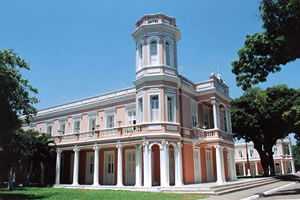
\includegraphics[width=16cm]{figuras/exemplo-1}
		}{
			\Fonte{\citeonline{UFC2012}.}
		}	
	\end{figure}
	
    Texto1 texto texto texto texto texto texto texto texto texto texto texto texto texto texto texto texto texto texto texto texto texto texto texto texto texto texto texto texto texto texto texto texto texto texto texto texto texto texto texto texto texto texto texto texto1.

    Texto2 texto texto texto texto texto texto texto texto texto texto texto texto texto texto texto texto texto texto. Texto texto texto texto texto texto texto texto texto texto texto texto texto texto texto texto texto texto texto2.

    Texto3 texto texto texto texto texto texto texto texto texto texto texto texto texto texto texto texto texto texto. Texto texto texto texto texto texto texto texto texto texto texto texto texto texto texto texto texto texto texto3.

    Texto4 texto texto texto texto texto texto texto texto texto texto texto texto texto texto texto texto texto texto. Texto texto texto texto texto texto texto texto texto texto texto texto texto texto texto texto texto texto texto4.

    A Figura \ref{fig:sondas} Texto texto texto texto texto texto texto texto texto texto texto texto texto texto texto texto texto texto texto. Texto texto texto texto texto texto texto texto texto texto texto texto texto texto texto texto texto texto texto3.

	\begin{figure}[h!]
		\centering
		\captionsetup{width=14cm}%Da mesma largura que a figura
		\Caption{\label{fig:sondas} Gráfico da Atmosfera Superior}	
		\UFCfig{}{
			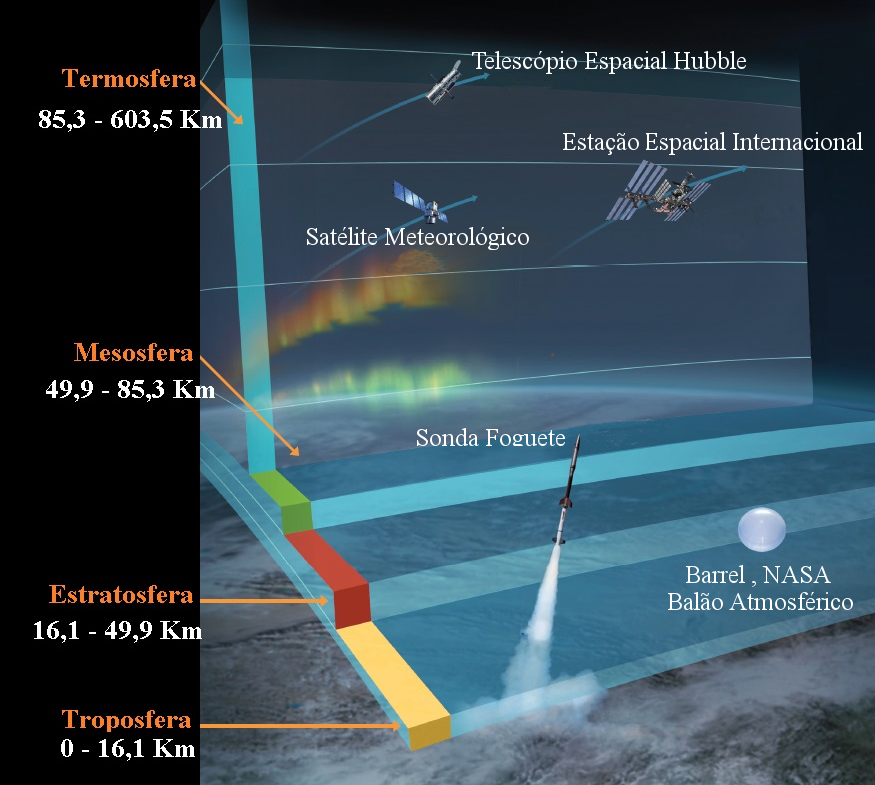
\includegraphics[width=14cm]{figuras/sondas}
		}{
			\Fonte{adaptado da \citeonline{NASA2016}.}}	
	\end{figure}

    Texto5 texto texto texto texto texto texto texto texto texto texto texto texto texto texto texto texto texto texto texto texto texto texto texto texto texto texto texto texto texto texto texto texto texto texto texto texto texto texto texto texto texto texto texto texto5.

    Texto6 texto texto texto texto texto texto texto texto texto texto texto texto texto texto texto texto texto texto texto texto texto texto texto texto texto texto texto texto texto texto texto texto texto texto texto texto texto texto texto texto texto texto texto texto5.

    Texto7 texto texto texto texto texto texto texto texto texto texto texto texto texto texto texto texto texto texto texto texto texto texto texto texto texto texto texto texto texto texto texto texto texto texto texto texto texto texto texto texto texto texto texto texto texto texto texto texto texto texto texto texto texto texto texto texto texto texto texto texto texto texto texto6.

    Evite terminar seções, capítulos e etc com figura. Procure escrever mais.

\section{Inserindo tabelas}\label{sec:tabelas}
    
    A Tabela \ref{tab:exemplo-1}... texto texto texto texto texto texto texto texto texto texto texto texto texto texto texto texto texto texto texto. Texto texto texto texto texto texto texto texto texto texto texto texto texto texto texto texto texto texto texto.
	
	\begin{table}[!h]
	\captionsetup{width=7cm}%Deixe da mesma largura que a tabela
	\Caption{\label{tab:exemplo-1} Um Exemplo de tabela alinhada que pode ser longa ou curta}%
	\IBGEtab{}{%
		\begin{tabular}{ccc}
			\toprule
			Nome & Nascimento & Documento \\
			\midrule \midrule
			Maria da Silva & 11/11/1111 & 111.111.111-11 \\
			Maria da Silva & 11/11/1111 & 111.111.111-11 \\
			Maria da Silva & 11/11/1111 & 111.111.111-11 \\
			\bottomrule
		\end{tabular}%
	}{%
	\Fonte{o autor.}%
	\Nota{esta é uma nota, que diz que os dados são baseados na
		regressão linear.}%
	\Nota[Anotações]{uma anotação adicional, seguida de várias outras.}%
    }
    \end{table}

	%\begin{table}[h!]	
	%	\centering
	%	\Caption{\label{tab:exemplo-1} Exemplo de tabela}	
	%	\UFCtab{}{
	%		\begin{tabular}{cll}
	%			\toprule
	%			Ranking & Exon Coverage & Splice Site Support \\
	%			\midrule \midrule
	%			E1 & Complete coverage by a single transcript & Both splice sites\\
	%			E2 & Complete coverage by more than a single transcript & Both splice sites\\
	%			E3 & Partial coverage & Both splice sites\\
	%			E4 & Partial coverage & One splice site\\
	%			E5 & Complete or partial coverage & No splice sites\\
	%			E6 & No coverage & No splice sites\\
	%			\bottomrule
	%		\end{tabular}
	%	}{
	%	\Fonte{elaborado pelo autor.}
	%}
	%\end{table}

\subsection{Exemplo de subseção} \label{sec:ex_sec}
	
    Texto texto texto texto texto texto texto texto texto texto texto texto texto texto texto texto texto texto texto texto texto texto texto texto texto texto texto texto texto texto texto texto texto texto texto texto texto texto texto texto texto texto texto texto texto.

    %acrlong{DATASUS},\acrlong{DNV},\acrlong{DO},\acrlong{ESF},\acrlong{IBGE},\acrlong{MFC},\acrlong{MI},\acrlong{MS},\acrlong{NV},\acrlong{ODM},\acrlong{OI},\acrlong{OMS},\acrlong{ONU},\acrlong{PNI},\acrlong{PSF},\acrlong{RIPSA},\acrlong{RN},\acrlong{SIM},\acrlong{SINASC},\acrlong{SUS},\acrlong{TMI},\acrlong{TMMFC}


    \begin{alineascomponto}
	    \item Integer non lacinia magna. Aenean tempor lorem tellus, non sodales nisl commodo ut
	    \item Proin mattis placerat risus sit amet laoreet. Praesent sapien arcu, maximus ac fringilla efficitur, vulputate faucibus sem. Donec aliquet velit eros, sit amet elementum dolor pharetra eget
	    \item Integer eget mattis libero. Praesent ex velit, pulvinar at massa vel, fermentum dictum mauris. Ut feugiat accumsan augue, et ultrices ipsum euismod vitae
	    \begin{subalineascomponto}
		    \item Integer non lacinia magna. Aenean tempor lorem tellus, non sodales nisl commodo ut
		    \item Proin mattis placerat risus sit amet laoreet.
	    \end{subalineascomponto}
    \end{alineascomponto}

\subsection{Uso de siglas} \label{sec:siglas}

    Para utilizar siglas, primeiro defina a sigla no arquivo "lista-de-abreviaturas-e-siglas"~ dentro da pasta "1-pre-textuais" com o comando 
    \begin{verbatim}
        \newacronym{ABNT}{ABNT}{Associação Brasileira de Normas Técnicas}
    \end{verbatim}
    Depois chame a sigla com o comando:
    \begin{verbatim}
        \gls{ABNT}
    \end{verbatim}
    Fica assim: \gls{ABNT}. A primeira vez que o comando é usado para uma determinada sigla, aparece o significado por extenso da sigla com a sua abreviação em seguida. A partir da segunda vez que o comando para uma determinada sigla é usado, aparace apenas a sigla. Por exemplo: \gls{ABNT}.  
    
    Veja o código fonte de outros exemplos: Teste de siglas \gls{TEST}, outros exemplos de siglas: \gls{DA}, \gls{MCEG}. 
    Repare que sempre as siglas estão sendo definidas primeiramente no arquivo ``lista-de-abreviaturas-e-siglas''.
\fi